\documentclass{article}
\usepackage[utf8]{inputenc}
\usepackage{amsmath, amssymb}
\usepackage[style=numeric, backend=biber]{biblatex}
\usepackage{graphicx}
\usepackage[breaklinks=true]{hyperref}
\addbibresource{references.bib}

\usepackage[a4paper, top=2.5cm, bottom=2.5cm, left=3cm, right=3cm]{geometry}
\DeclareFieldFormat{urldate}{
    (accessed on \thefield{urlday}/\thefield{urlmonth}/\thefield{urlyear})
}
\hypersetup{
    colorlinks=true,
    pdfborder={0 0 0},
    linkcolor=blue,   % internal links
    citecolor=magenta,  % citations
    urlcolor=blue     % URLs
}

\title{Number and Group Theory\\\textbf{TC50331E}\\Algebraic Coding Theory}
\author{Jaish Singh\\33139652}
\date{April 2026}

\begin{document}
\maketitle
\setlength{\parskip}{0.5cm}

Every time data travels across a network, a file being downloaded or a being message sent, there is 
a chance that some bits flip to the opposite sign. The challenge of reliable communication is therefore 
not only one of engineering, but of mathematics. How do we design systems that can detect and correct 
errors, without knowing in advance where they will occur? Algebraic coding theory answers this question 
by imposing carefully chosen mathematical structure on transmitted data. This report develops the theory 
of binary block codes, showing how group theory provides the natural language for describing and 
detecting errors.

\section{Block Codes}

%-----------------------------  1 (a)  -----------------------------
Let \(\mathbf{B}(n) = \underbrace{\mathbb{Z}_2 \times \mathbb{Z}_2 \times \cdots \times 
\mathbb{Z}_2}_{n \text{ copies}}\), the set of all binary strings of length \(n\). That is,
\[
    \mathbf{B}(n) = \{ (x_1, \dots, x_n) \mid x_i \in \mathbb{Z}_2 \text { for }
  1 \le i \le n \}.
\]
We equip this set with a binary component-wise addition in modulo 2: 
\[ (x_1, \dots, x_n) + (y_1, \dots, y_n) = (x_1 + y_1, \dots, x_n + y_n)\]
where addition is taken in $\mathbb{Z}_2$. This operation is well-defined 
since \( \mathbb{Z}_2 \) is closed under addition. We verify the group axioms 
for \((\mathbf{B}(n), + )\):
\begin{enumerate}
    \item \textit{Closure: } Let \( x, y \in \mathbf{B}(n) \). Then \( x + y \in \mathbf{B}(n) \) 
        since addition in \( \mathbb{Z}_2 \) is closed.

    \item \textit{Associativity: } For all \( x, y, z \in \mathbf{B}(n) \), we have
    \[ (x + y) + z = x + (y + z), \] since addition in
    \( \mathbb{Z}_2 \) is associative.

\item \textit{Identity: } The element \( 0 = (0, \dots, 0) \in \mathbf{B}(n) \) satisfies 
    \( x + 0 = x \) for all \( x \in \mathbf{B}(n) \).

\item \textit{Inverses: } For each \( x \in \mathbf{B}(n) \), we have \( x + x = 0 \) since 0 + 0 = 0
    and 1 + 1 = 0, so every element is its own inverse.
\end{enumerate}
Having established that \( (\mathbf{B}(n), +) \) is a group, we observe that it is in
fact Abelian. This follows from the commutativity of addition in \( \mathbb{Z}_2 \), 
applied component-wise. Since digital signals are inherently binary, it is natural to 
model transmitted data as elements of \(\mathbb{Z}_2 = \{0, 1\}\), the group of integers
modulo 2 under addition. The group operation, which coincides with XOR, captures parity 
computations precisely: the parity of a binary string is simply its sum in \(\mathbb{Z}_2\).
This structure extends naturally to \(\mathbb{Z}_2^n\), the group of binary strings of 
length n, which serves as the space in which code words live. 

%-----------------------------  1 (b)  -----------------------------
For \(0 < k < n\), we define an \((n, k)\) block code to be a subset of \(\mathbf{B}(n)\), 
such that the cardinality of the block code \((n, k) = 2^k\), and elements are binary strings, called code 
words, of length \(n\). We restrict transmission of binary data to only the code words within the prescribed 
block code. Since bit flips can happen seemingly at random, the code words may get transformed to binary 
strings outside the block code. Hence, the received words are elements of a broader set of all binary strings 
of length \(n\), \(\mathbf{B}(n)\). Additionally, if a block code happens to be a subgroup of \(\mathbf{B}(n)\),
then this is a special type of block code called a Linear Block Code. Linear Block Codes have several
structural qualities, explored in more depth in the subsequent sections, that make them more efficient. 

For instance, consider a set \(C = \{(0,0,0,0), (0,1,0,1), (1,0,1,0), (1,1,1,1)\}\). \(C\) is a (4, 2) block 
code since every code word is of length 4 and \(|C| = 4 = 2^2\) corresponding to \(k=2\) information bits. 
Since transmission may cause errors anywhere in the string, the received words for any element in \(C\) 
are all binary strings of length 4, i.e. any element in \(\mathbf{B}(4) =\) \{0000, 0001, 0010, 0011, 0100, 
0101, 0110, 0111, 1000, 1001, 1010, 1011, 1100, 1101, 1110, 1111\}. For \(a, b \in C\), \(a + b^{-1} \in C\),
which establishes that \(C\) is a subgroup of \(\mathbf{B}(4)\), and therefore \(C\) is a Linear Block Code.

%-----------------------------  1 (c & d)  -----------------------------

A generator matrix \(\mathbf{G}\), for a \((n, k)\) block code \(C\) is a \(k \times n\) matrix whose rows form 
a basis for \(C\), i.e. are linearly independent. We use a generator matrix \parencite{berlekamp1972survey} to 
systematically generate code words in a block code. For instance, the generator matrix \(\mathbf{G}\), for a 
\((5, 2)\) block code \(C = \{(0,0,0,0,0), (1,0,1,1,0), (0,1,1,0,1), (1,1,0,1,1)\}\) is defined as
\[\mathbf{G} = \begin{pmatrix} 
    1 & 0 & 1 & 1 & 0 \\
    0 & 1 & 1 & 0 & 1 \\
\end{pmatrix}\]
To verify if a received word is a valid code word, we make use of a \((n-k) \times n\) parity-check matrix,
\(H\). The valid code words are the null space of the parity-check matrix, i.e., \[HG^T = 0\]
Similarly, a received word \(C\) is a valid code word if it satisfies the equation \( HC^T = 0 \).
The parity-check matrix, \(H\), for our \((5, 2)\) block code is

\[
H = \begin{pmatrix}
1 & 0 & 0 & 1 & 0 \\
0 & 1 & 0 & 0 & 1 \\
0 & 0 & 1 & 1 & 1
\end{pmatrix}\]

\[
HG^T = \begin{pmatrix}
1 & 0 & 0 & 1 & 0 \\
0 & 1 & 0 & 0 & 1 \\
0 & 0 & 1 & 1 & 1
\end{pmatrix}
\begin{pmatrix}
1 & 0 \\
0 & 1 \\
1 & 1 \\
1 & 0 \\
0 & 1
\end{pmatrix}
= 
\begin{pmatrix}
0 & 0 \\
0 & 0 \\
0 & 0
\end{pmatrix}
\]

%-----------------------------  1 (e)  -----------------------------
For a given block code, we must define its capabilities in terms of error detection and error
correction. This capability is defined in terms of the \textit{weight} of a code word in a 
block code. The weight of a binary string \(b \in \mathbf{B}(n)\), denoted by \(w(b)\), is the count of
1s in \(b\). For instance, the weight of \((1,0,1,1,0,1,1,0,1,1,0,1) \in \mathbf{B}(12)\) is 8.
%-----------------------------  1 (f)  -----------------------------
The \textit{distance} \(d\), between two binary strings, \(x , y \in \mathbf{B}(n)\), is the weight of their 
sum in \(\mathbb{Z}_2\), i.e., 
\[d(x, y) = w(x + y)\]
In other words, the distance is the number of positions where the two strings differ.
The distance defines a metric \parencite{hamming1950error} on \(\mathbf{B}(n)\). Formally, a metric defined on a 
set is a function such that it follows
\begin{enumerate}
\item Definiteness: \(d(x, y) = 0 \iff x = y\)
\item Symmetry: \(d(x, y) = d(y, x)\)
\item Triangle inequality: \(d(x, z) \leq d(x, y) + d(y, z)\)
\end{enumerate}
It is straightforward to verify that \(d\) satisfies each of these.
\begin{enumerate}
    \item Definiteness: \(d(x,y) = w(x + y) = 0\) if and only if \(x + y = 0\), which holds 
        if and only if \(x_i = y_i\) for all \(i\), i.e. \(x = y\).

    \item Symmetry: \(d(x,y) = w(x + y) = w(y + x) = d(y,x)\), since \(x_i + y_i = y_i 
        + x_i\) for each bit.

    \item Triangle inequality: For any \(x, y, z \in \mathbf{B}(n)\), note that
        \begin{align*}
            (x + z) &= x + 0 + z \\
                    &= x + (y + y) + z \\
                    &= (x + y) + (y + z) \\
        \end{align*}
        so,
        \begin{align*}
            d(x,z) &= w(x+ z) \\
                   &= w\bigl((x + y)+(y + z)\bigr) \leq w(x + y) + w(y + z) \\
                   &= d(x,y)+d(y,z) \\
        \end{align*}
        where the inequality uses subadditivity of weight: \((a + b)_i = 1\) only if \(a_i = 1\) or \(b_i = 1\),
        so every position counted in \(w(a + b)\) is also counted in \(w(a) + w(b)\), giving \(w(a + b) \leq w(a) + w(b)\).
\end{enumerate}
This metric structure carries directly into the analysis of block codes, where distance between codewords
becomes the central quantity of interest.

\section{Decoding and Errors}
%-----------------------------  2 (a)  -----------------------------
Let \(C\) be a code word to be transmitted, and \(R\) its received counterpart. The error in
transmission is measured by the distance between the sent binary string and the received 
string, \(d(C, R)\). These errors change the message seemingly at random coordinates, and therefore,
there is a non zero chance for the received message to have been transformed to another valid code 
word. If \(C\) is corrupted by \(e\) errors, \(R\) lies at a distance \(e\) from \(C\). Let \(d_\text{min}\)
be the smallest distance between any two valid code words in a block code. Provided \(e < d_\text{min}\),
the received word cannot coincide with any other valid codeword. Therefore the decoder can detect up to 
\(d_\text{min} - 1\) errors. If \(R\) is detected to have errors, it may be possible to error correct the message.
We simply do this by taking the nearest valid code word to \(R\) as the intended message. 


Correction is possible only when \(R\) has a unique nearest codeword, i.e., it is not equidistant between two 
codewords. Conversely, \(R\) must be at most \(\lfloor\frac{d_\text{min} - 1}{2}\rfloor\) from a valid code word,
where \(\lfloor \cdot \rfloor\) denotes the floor function, rounding down to the nearest integer. Therefore,
a code with minimum distance \(d_\text{min}\) can correct at most \(\lfloor\frac{d_\text{min} - 1}{2}\rfloor\)
errors, since any \(R\) within that radius is guaranteed to be closer to exactly one valid code word than any
other. In other words, \(d_\text{min} \geq 2t + 1\) \parencite{bose1960class}, where \(t\) is the number of errors 
the block code can correct.
Conversely, suppose for contradiction that a block code \(\mathbf{C}\) corrects \(t\) errors but \(d_\text{min} 
\leq 2t\). Then there exist distinct codewords \(C_1, C_2 \in \mathbf{C}\) with \(d(C_1, C_2) \leq 2t\). We 
construct \(R\) by flipping \(\lfloor \frac{d(C_1, C_2)}{2} \rfloor\) bits of \(C_1\) toward \(C_2\). Then 
\(d(R, C_1) \leq t\) and \(d(R, C_2) \leq t\), so nearest-neighbour decoding cannot uniquely recover the 
original code word. This contradicts our assumption, therefore we establish that a block code can recover 
\(t\) errors if and only if \(d_\text{min} \geq 2t + 1\).

%-----------------------------  2 (b)  -----------------------------
Let G be a block code described by
\[
G = \begin{pmatrix}
    1 & 0 & 0 & 1 & 1 & 1 \\
    0 & 1 & 0 & 1 & 0 & 1 \\
    0 & 0 & 1 & 1 & 1 & 0 \\
\end{pmatrix}
\]
where the code words for G are defined by the encoding algorithm 
\begin{align*}
\mathbf{C} &= \{B\mathbf{G} : B \in \mathbf{B}(3)\} \subset \mathbf{B}(6)\} \\
           &= \{000000,\ 100111,\ 010101,\ 001110,\ 110010,\ 101001,\ 011011,\ 111100\}
\end{align*}
Since \(\mathbf{C}\) is closed under addition in \(\mathbb{Z}_2\) and contains 000000, \(\mathbf{C}\) 
is a group and consequently a Linear Block Code. As a result, for any two code words \(C_1, C_2 \in \mathbf{C}\),
their sum \(C_1 + C_2 \in \mathbf{C}\), and the distance satisfies \(d(C_1, C_2) = w(C_1 + C_2)\).
Therefore \(d_\text{min}\), the smallest distance between any two valid code words, would be the 
smallest weight of a codeword in \(\mathbf{C}\) excluding 000000, which by inspection we deduce to be 3, 
the weight of 010101. Using \(d_\text{min}\), we infer that \(\mathbf{G}\) can detect at most 
\(d_\text{min} - 1 = 2\) errors and correct \(\lfloor\frac{d_\text{min} - 1}{2}\rfloor = 1\)
error.

%-----------------------------  2 (c) -----------------------------
The parity-check matrix, \(\mathbf{H}\), validates any input \(B \in \mathbf{B}(n)\) given by
\(F: \mathbf{B}(n) \rightarrow \mathbf{B}(n - k)\) such that,
\[
    F(B) = \mathbf{H}B^t, B \in \mathbf{B}(n)
\]
If an error is detected, we take the nearest valid code word to be the message. However, to search 
for the nearest valid code word by individually measuring the distance between every possible word 
would be computationally expensive. To get around this, we use the fact that \(F\) is a surjective
group homomorphism. Since \(F\) satisfies the condition \(F(a + b) = F(a) + F(b)\) which follows from the 
linearity of matrix multiplication, \(F\) is a group homomorphism. We also know that \(\mathbf{H}\) has a 
full row rank \(n - k\) which is an inherent property of \(\mathbf{H}\) by the definition of a parity-check
matrix. This suggests that the linear map \(F\) can produce any vector in \(\mathbf{B}(n - k)\) and 
therefore is a surjective map. Thus, we deduce that \(F\) is a surjective group homomorphism, which allows 
us to partition \(\mathbf{B}(n)\) into cosets of the kernel of \(F\).
\[
F(B) = HB^t = H(C + e)^t = HC^t + He^t = 0 + He^t = He^t
\]
where \(e\) is the error in \(B\). We precompute all cosets of the kernel of \(F\) in \(\mathbf{B}(n)\) and 
find the element with the smallest weight in each coset, called the coset leader, \(\hat{e}\). When 
decoding, we find the coset in which \(F(B) = He^t\) belongs to in our precomputed set of cosets. Once 
we have found our coset, and its corresponding coset leader \(\hat{e}\), finding the closest 
code word \(\hat{C}\) becomes trivial
\[
    \hat{C} = B + \hat{e}
\]
Since \(F\) is a group homomorphism, its kernel \(ker(F) = \{B \in \mathbf{B}(n):\mathbf{H}B^t = 0\}\) is
a subgroup of \(\mathbf{B}(n)\). Because \(\mathbf{HG}^t = 0\), every codeword \(C = B\mathbf{G}\) satisfies 
\(F(C) = \mathbf{H}C^t = 0\), so all valid codewords lie in \(\ker(F)\). Conversely, any \(B \in \ker(F)\) 
satisfies \(\mathbf{H}B^t = 0\) and therefore belongs to the block code. Hence \(B \in \mathbf{B}(n)\) is a 
codeword if and only if \(\mathbf{H}B^t = 0\).

%-----------------------------  2 (d) -----------------------------
A natural follow up to this is understanding how efficiently we can encode information, i.e., given a block length 
\(n\), how many information bits \(k\) can we transmit while still correcting \(t\) errors? Since \(|C| = 2^k\), 
bounding the number of codewords directly bounds \(k\). Each codeword \(C\) occupies a sphere of radius \(t\), 
containing \(\sum_{i=0}^{t}\binom{n}{i}\) elements of \(\mathbf{B}(n)\). Since these spheres must be disjoint,
\(|C| \cdot \sum_{i=0}^{t}\binom{n}{i} \leq 2^n\). For \(t=1\) this gives \(2^k(1+n) \leq 2^n\), or equivalently
\(k \leq n - \log_2(1+n)\) \parencite{berlekamp1972survey}.
A Hamming code is a linear block code that achieves exactly this bound. Therefore every element of 
\(\mathbf{B}(n)\) lies in exactly one decoding sphere. Formally, a Hamming code with redundancy \(m\)
has parameters \(n = 2^m - 1\), \(k = 2^m - 1 - m\), with the parity-check matrix \(H\) having dimensions
\(m \times (2^m-1)\). Since no column of \(H\) is zero and no two columns are the same, no codeword of weight 
1 or 2 can exist (since \(HB^t = 0\) would require a 0 column or two identical columns). Thus, \(d_\text{min}
\geq 3\). Since three columns can sum to zero (for instance, any column $h_i$ satisfies $h_i + h_j + (h_i + h_j)
= 0$ for distinct $i, j$, and $h_i + h_j$ is itself a non-zero column of $H$), some weight-3 codeword exists,
giving \(d_\text{min} = 3\) exactly \parencite{hamming1950error}.

A received word \(B\) is a valid codeword if and only if \(HB^T = 0\). If a single-bit error occurs at position 
\(i\), the syndrome \(HB^t\) equals precisely the \(i^\text{th}\) column of \(H\), which uniquely identifies 
the coset containing \(B\). Since each single-bit error vector is the coset leader of a distinct coset, 
guaranteed by the fact that all columns of \(H\) are distinct and non-zero, we can recover \(\hat{e}\) directly
from the syndrome, making the lookup into our precomputed coset table trivial.

\section{Empirical Investigation}
%-----------------------------  3 (a) -----------------------------
\subsection{Setup}
The simulation \parencite{jaish2026} consists of a \texttt{Block\_code} class that takes codewords
$\mathbf{C} \subseteq \mathbf{B}(n)$ as input. From the list of code words, we determine 
$k = \log_2 |\mathbf{C}|$. We assume the input to be valid and a linear block code 
and therefore $C$ to be a subgroup of $\mathbf{B}(n)$. Since we are dealing with linear block codes,
the distance between any two codewords $C_1, C_2 \in \mathbf{C}$ satisfies $d(C_1, C_2) = w(C_1 + C_2)
\in \mathbf{C}$. We use this to compute $d_\text{min}$ by calculating the weight of each code word. 
The error-detection and correction capacities are then computed as $d_{\min} - 1$ and $\lfloor 
\frac{d_{\min}-1}{2} \rfloor$, respectively.

Encoding is described by the matrix product $C = \mathbf{m} \cdot G$. Here, $\mathbf{m}$ is a list of 
length $k$ containing the message in binary format. $C$ is the resulting codeword of length $n$, and $G$ is 
the $k \times n$ generator matrix derived from $\mathbf{C}$ via Gaussian elimination. 
\texttt{compute\_generator\_matrix} row-reduces the entire list of codewords to identify $k$ linearly
independent rows, resulting in $G$ in systematic form $[I_k \mid P]$. The parity-check matrix is then
computed algebraically as $H = [P^T \mid I_{n-k}]$, which follows $HG^T = 0$ by design.

When initializing the block code, we run \texttt{compute\_syndrome\_table} to systematically compute all error
patterns and their corresponding syndrome in order of increasing weight. The first error pattern computed for 
each syndrome is recorded as the coset leader $\hat{e}$. The table is complete when it has $2^{n-k}$ entries, since 
$\mathbf{B}(n)$ divides into exactly $2^{n-k}$ cosets of $\mathbf{C}$, as shown by the surjectivity of 
$F(B) = HB^T$. During runtime, \texttt{correct} computes the syndrome of the received word with simulated 
random errors. By matching the syndrome with the coset leaders in the syndrome table, we find the corresponding 
error pattern. We then add this error pattern to $R$ since the inverse of the error is itself. This 
subsequently outputs the corrected codeword ($\hat{\mathbf{C}} = R + \hat{e}$). If the weight of the coset 
leader is larger than $\lfloor \frac{d_{\min}-1}{2} \rfloor$, an error is raised because reliable correction 
is not guaranteed. Note that while generating the syndrome table is expensive since we compute every 
error pattern possible for the block code, this is only done once at initialization which allows us to have very 
inexpensive correction of received words at runtime.

We define \texttt{send}, to randomly add error to a code word. \texttt{send} takes a codeword and an error count.
It randomly picks positions in the binary string to flip to the opposite sign. 
We simulate the transmission scenario described in Section 2. A codeword $\mathbf{C}$ is sent, random errors occur,
and a received word $R$ comes back with simulated errors. We use this to observe characteristics of block codes
empirically.

One limitation of this implementation is that \texttt{compute\_syndrome\_table} has a memory cost 
of $O(2^{n-k})$, which can become problematic for large $n$. Additionally, \texttt{send} assumes
errors happen independently at random positions, which is an idealized assumption. In reality, 
errors may cluster together, affecting more positions than the model expects.

%-----------------------------  3 (b) -----------------------------
\subsection{Experiment}
We systematically vary \(n\) and \(k\) for a block code to observe changes in \(d_\text{min}\).
We use \(d_\text{min}\) as a proxy for our block codes' utility since both error correction as well as error 
detection capacity of a block code are computed using \(d_\text{min}\), where larger \(d_\text{min}\) relates to 
better error-control capabilities.

\begin{figure}[ht]
    \centering
    \noindent
    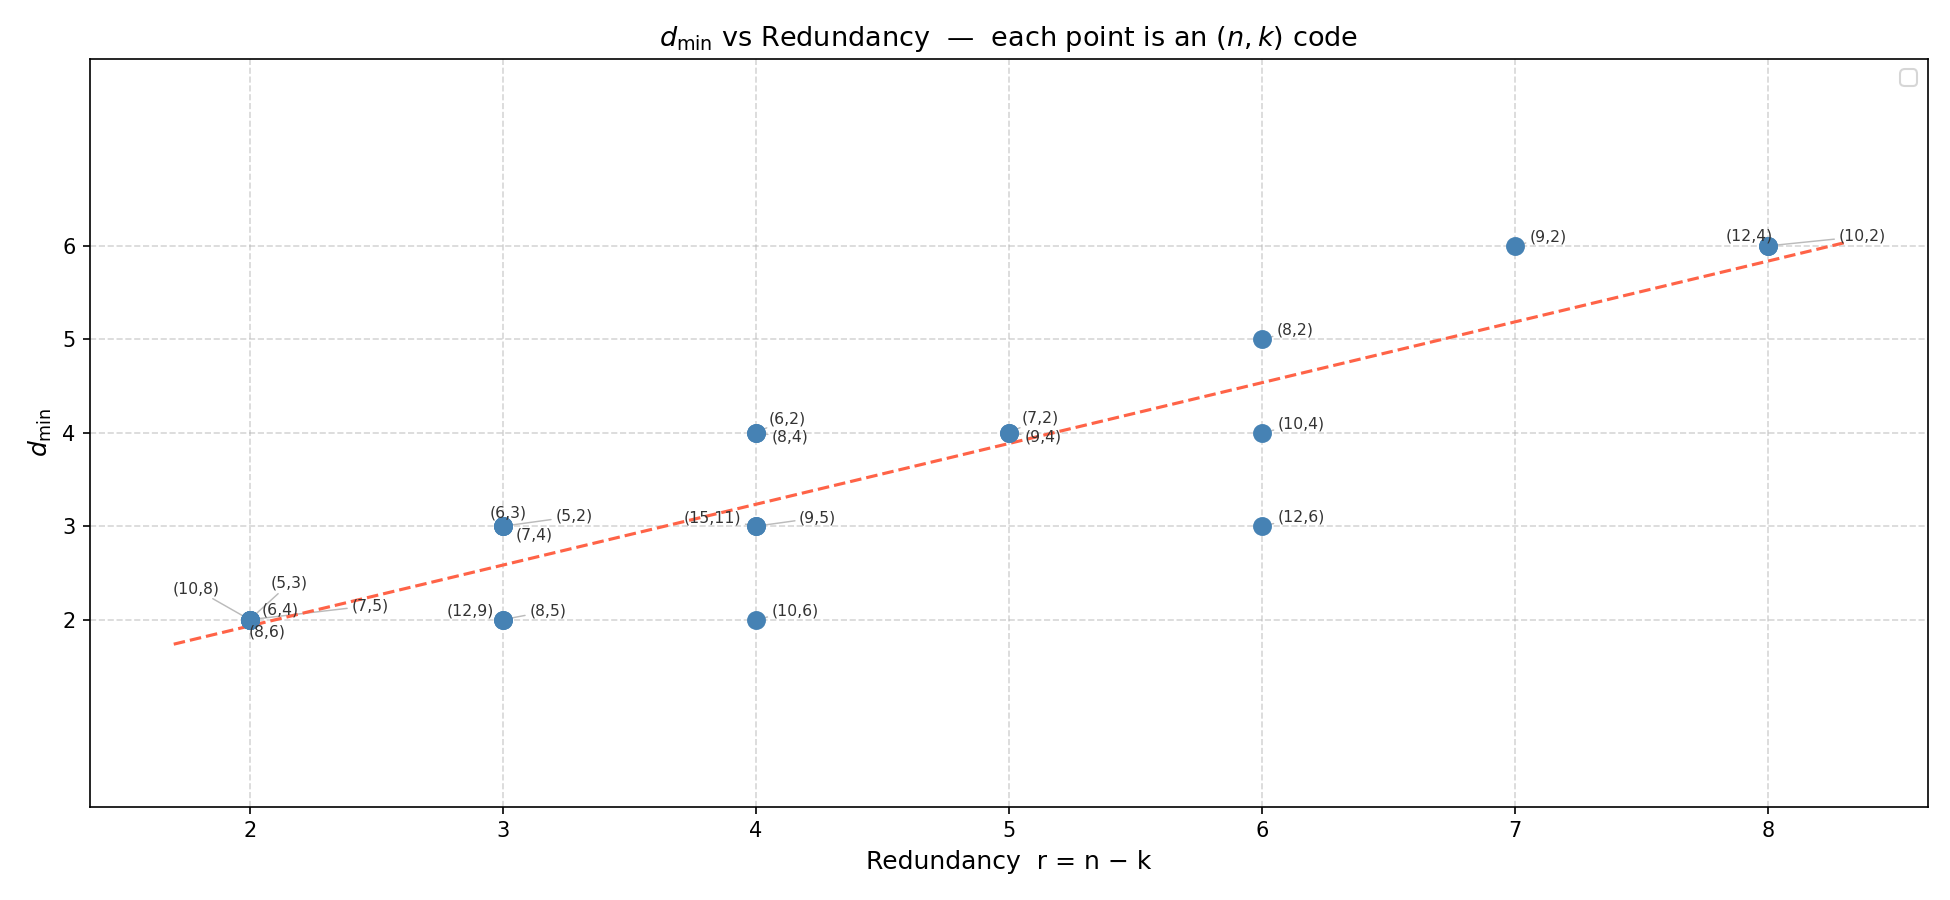
\includegraphics[width=\linewidth]{dmin_vs_redundancy.png}
    \caption{\(d_\text{min}\) vs Redundancy for varying block codes}
    \label{fig:d_min_vs_Redundancy}
\end{figure}

The scatter plot confirms a positive trend between redundancy \(r = n - k\) and \(d_\text{min}\): as more 
redundant bits are added, larger \(d_\text{min}\) becomes achievable. However, the vertical scatter at 
each value of \(r\) suggests that while redundancy is a necessary condition for \(d_\text{min}\), it does not fully
explain \(d_\text{min}\). At \(r = 4\), \(d_\text{min}\) varies from 2 for the (10,6) block code to 4 for (6,2). 
The (15,11) Hamming code is a significant point of interest: it attains \(d_\text{min} = 3\) at \(r = 4\) while 
encoding 11 information bits. This highlights that the structure of a block code is a significant factor when
assessing its utility. The dashed trend line captures the general correlation between \(d_\text{min}\) and \(r\),
but the scatter around it emphasizes that choosing a block code requires optimising construction, not just increasing
redundancy.

\begin{figure}[ht]
    \centering
    \noindent
    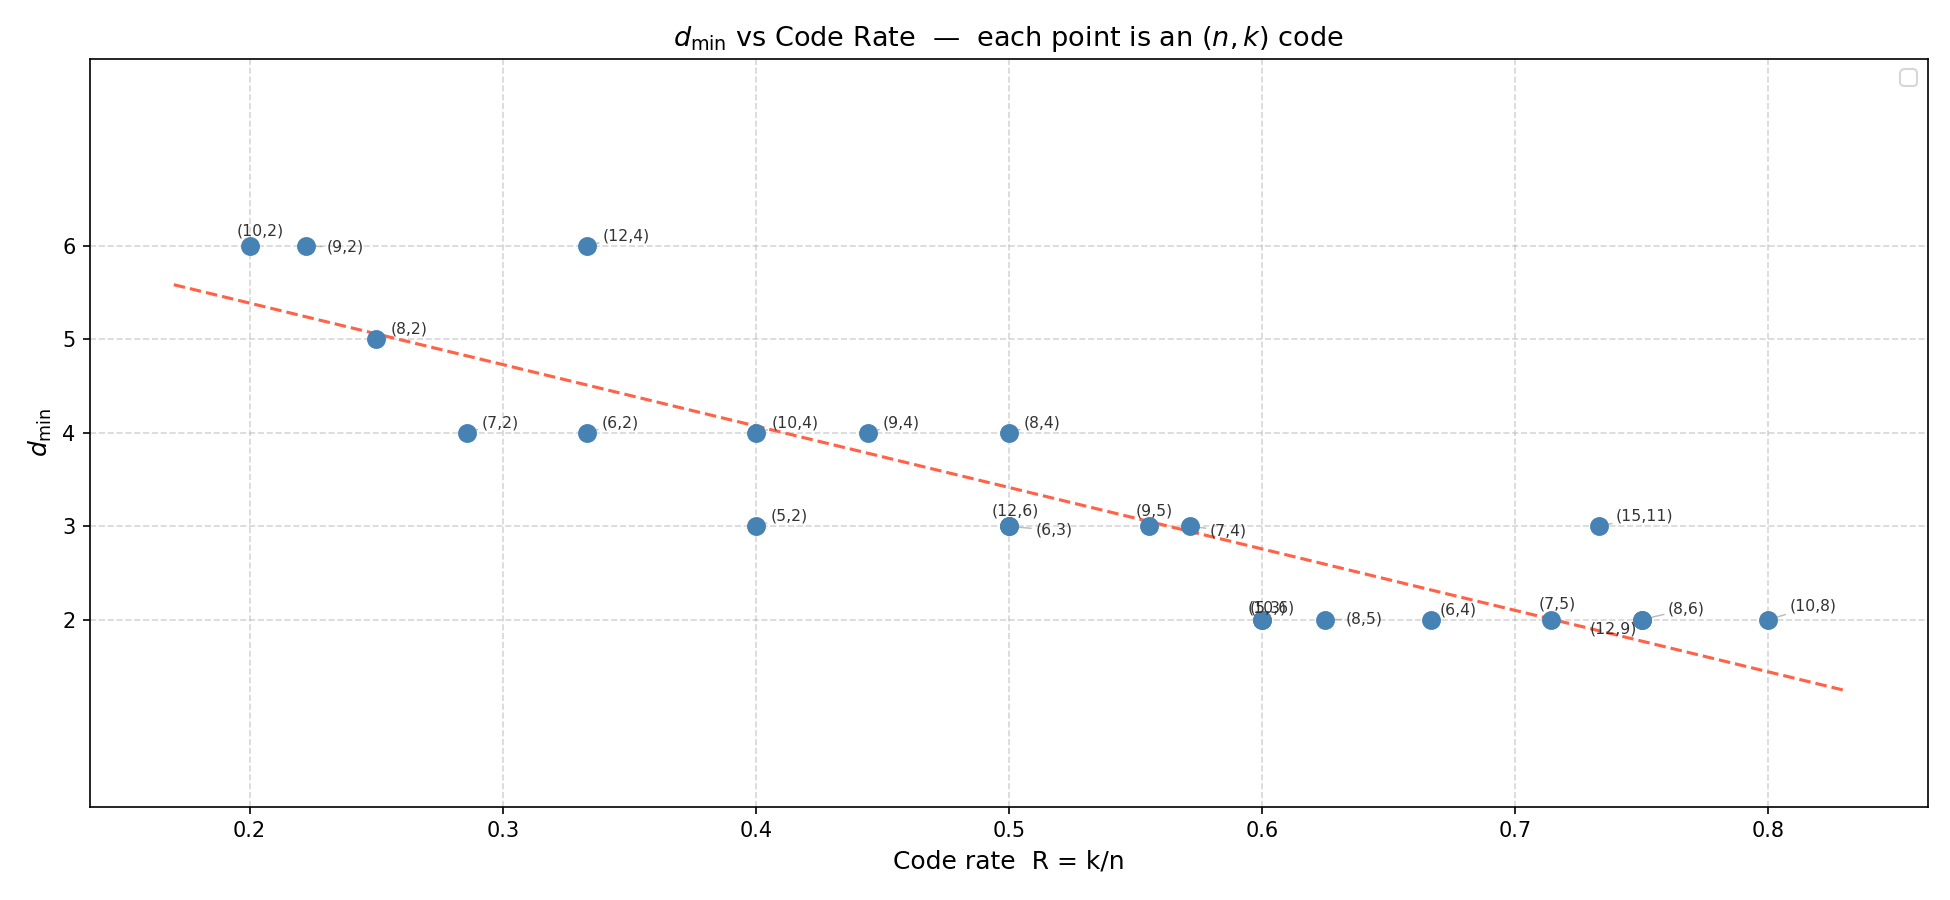
\includegraphics[width=\linewidth]{dmin_vs_rate.png}
    \caption{\(d_\text{min}\) vs Code Rate for varying block codes [\autoref{tab:empirical_investigation}]}
    \label{fig:d_min_vs_Rate}
\end{figure}

Figure 2 confirms the underlying antagonism between code rate \(R = k/n\) and error-correction capacity. As \(R\) 
increases, the achievable \(d_\text{min}\) falls. The negative trend is prominent, but the scatter around it again 
shows that rate alone does not fully explain \(d_\text{min}\). We notice that the (12,4) block code is a significant 
outlier, attaining \(d_\text{min} = 6\) at \(R \approx 0.33\), well above comparable code rates, highlighting how longer 
block lengths can achieve greater distance at the same rate. At the high-rate end, the (15,11) Hamming code stands out 
for attaining \(d_\text{min} = 3\) at \(R \approx 0.73\), an area where most block codes max out at \(d_\text{min} = 2\).
A noticeable floor at \(d_\text{min} = 2\) appears for \(R \ge 0.6\), suggesting that beyond this threshold, further 
increases in code rate do not meaningfully worsen \(d_\text{min}\). This indicates that \(d_\text{min}\) is 
already at its practical minimum. The widest vertical scatter appears at low \(R\), indicating that block codes with low
\(R\) offer the greatest design flexibility, while block codes with high \(R\) converge toward the minimum distance floor.

\begin{figure}[ht]
    \centering
    \noindent
    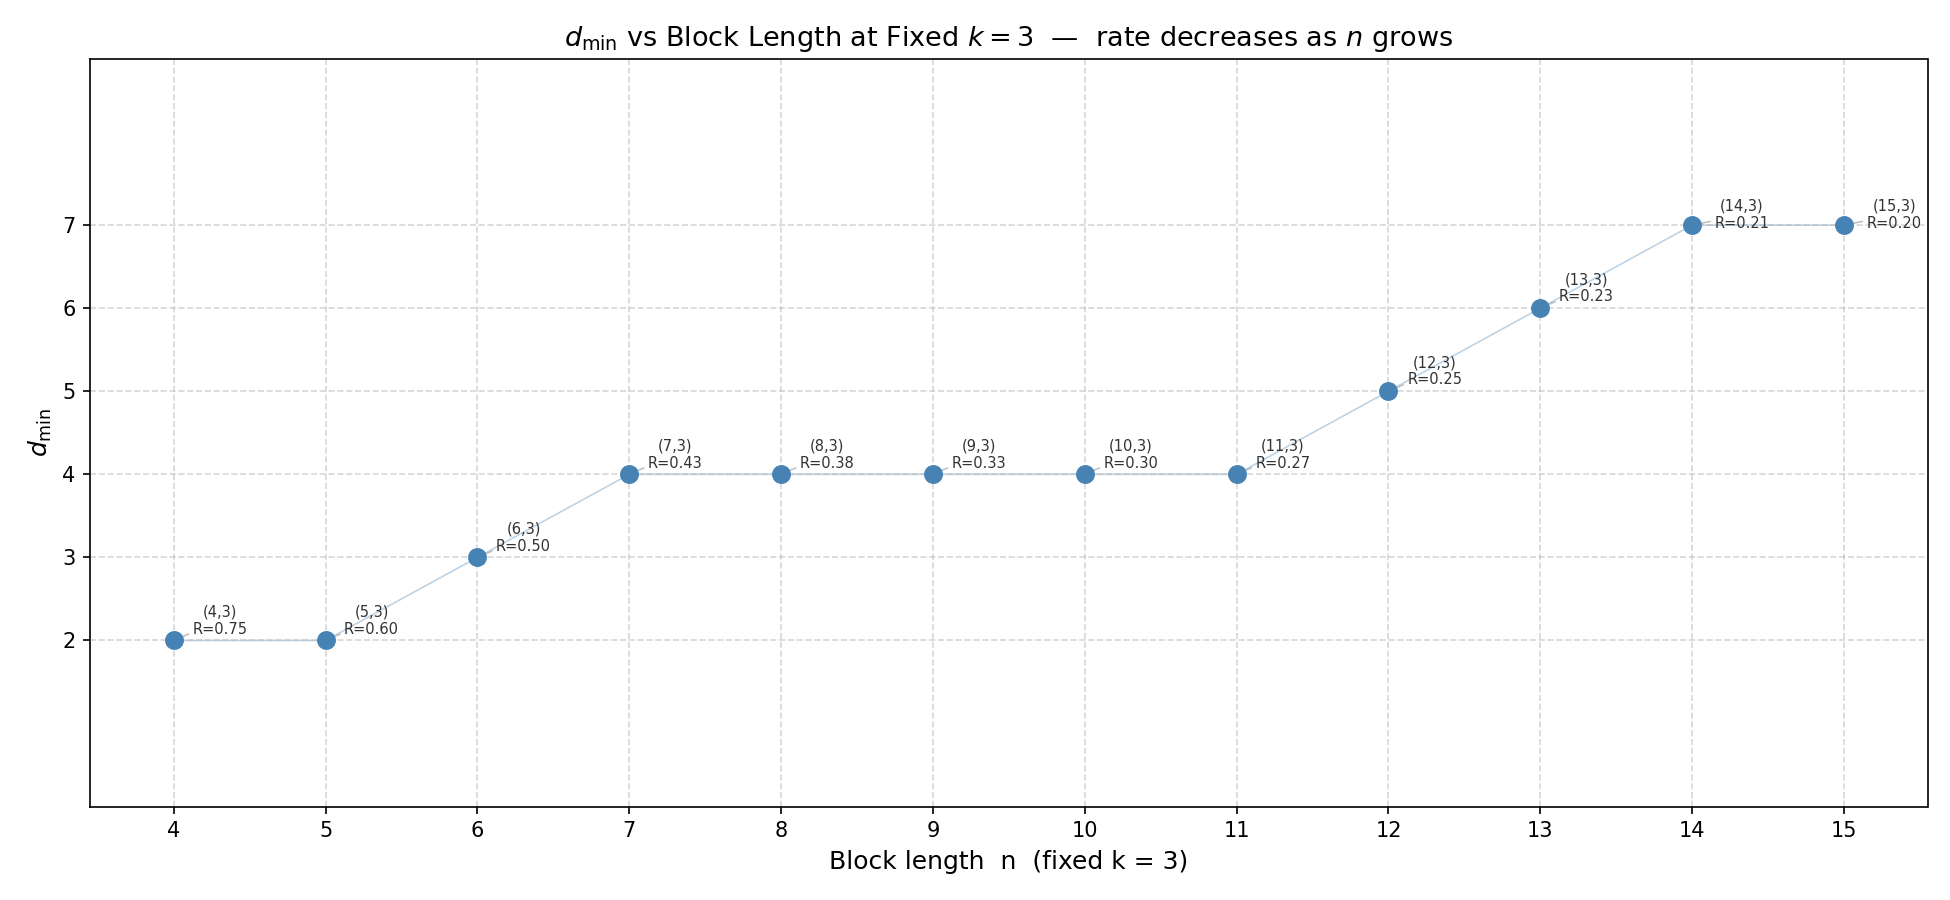
\includegraphics[width=\linewidth]{dmin_vs_n_fixed_k.png}
    \caption{\(d_\text{min}\) vs n for fixed k [\autoref{tab:fixed_k}]}
    \label{fig:d_min_vs_n}
\end{figure}

With \(k\) fixed at 3, increasing the block length \(n\) is equivalent to adding redundancy while holding information 
bits constant, and Figure 3 shows that this reliably grows \(d_\text{min}\), but not linearly. The progression is 
distinctly step-wise, \(d_\text{min}\) increases are separated by flat plateaus, reflecting the discrete geometry of 
Hamming space rather than a continuous trade-off. The most notable plateau spans from \(n = 7\) to \(n = 11\), where 
five block codes share \(d_\text{min} = 4\) even as the \(R\) falls from 0.43 to 0.27, four extra redundant 
bits that result in no improvement in \(d_\text{min}\). The escape from the plateau at \(n = 12\) suggests that increases 
in distance are unlocked only at specific thresholds, making naive redundancy addition an inefficient design strategy.

Figures 1-3 give a coherent and practically important picture of block code design. Figure 1 establishes that 
redundancy is a prerequisite for large \(d_\text{min}\), but construction quality determines how efficiently that 
redundancy is converted. Figure 2 reframes the same trade-off through code rate, revealing a \(d_\text{min}\)
floor at high rates and the greatest design freedom at low rates. Figure 3 isolates block length, even with \(k\) fixed,
increases in \(d_\text{min}\) are not proportional to added redundancy. They arrive in discrete steps, with long 
plateaus where extra bits are effectively wasted. Across all three perspectives, the conclusion is the same, parameter 
choices set the ceiling on achievable \(d_\text{min}\), but it is the algebraic structure of the code that determines 
whether that ceiling is approached. Efficient block code design is therefore not just a matter of allocating more 
bits to redundancy, but of constructing codes whose geometry exploits every redundant bit to maximally separate 
codewords.

\newpage
\centering
\printbibliography

\appendix
\section{Appendix}
\begin{table}[ht]
  \centering
  \begin{tabular}{ccccc}
    \hline
    \(n\)  &  \(k\)  &  Redundancy \((n - k)\)  & code rate \((k/n)\) & \(d_\text{min}\)\\
    \hline
         5  &   2  &  3  &  0.40  &  3 \\
         5  &   3  &  2  &  0.60  &  2 \\
         6  &   2  &  4  &  0.33  &  4 \\
         6  &   3  &  3  &  0.50  &  3 \\
         6  &   4  &  2  &  0.67  &  2 \\
         7  &   2  &  5  &  0.29  &  4 \\
         7  &   4  &  3  &  0.57  &  3 \\
         7  &   5  &  2  &  0.71  &  2 \\
         8  &   2  &  6  &  0.25  &  5 \\
         8  &   4  &  4  &  0.50  &  4 \\
         8  &   5  &  3  &  0.63  &  2 \\
         8  &   6  &  2  &  0.75  &  2 \\
         9  &   2  &  7  &  0.22  &  6 \\
         9  &   4  &  5  &  0.44  &  4 \\
         9  &   5  &  4  &  0.56  &  3 \\
        10  &   2  &  8  &  0.20  &  6 \\
        10  &   4  &  6  &  0.40  &  4 \\
        10  &   6  &  4  &  0.60  &  2 \\
        10  &   8  &  2  &  0.80  &  2 \\
        12  &   4  &  8  &  0.33  &  6 \\
        12  &   6  &  6  &  0.50  &  3 \\
        12  &   9  &  3  &  0.75  &  2 \\
        15  &  11  &  4  &  0.73  &  3 \\
    \hline
  \end{tabular}
  \caption{\(d_\text{min}\) for block codes of varying n and k \parencite{jaish2026}}
  \label{tab:empirical_investigation}
\end{table}

\begin{table}[ht]
  \centering
  \begin{tabular}{ccccc}
    \hline
    \(n\)  &  \(k\)  &  Redundancy \((n - k)\)  & code rate \((k/n)\) & \(d_\text{min}\)\\
    \hline
         4  &  3  &   1  &  0.75  &  2 \\
         5  &  3  &   2  &  0.60  &  2 \\
         6  &  3  &   3  &  0.50  &  3 \\
         7  &  3  &   4  &  0.43  &  4 \\
         8  &  3  &   5  &  0.38  &  4 \\
         9  &  3  &   6  &  0.33  &  4 \\
        10  &  3  &   7  &  0.30  &  4 \\
        11  &  3  &   8  &  0.27  &  4 \\
        12  &  3  &   9  &  0.25  &  5 \\
        13  &  3  &  10  &  0.23  &  6 \\
        14  &  3  &  11  &  0.21  &  7 \\
        15  &  3  &  12  &  0.20  &  7 \\
    \hline
  \end{tabular}
  \caption{\(d_\text{min}\) for fixed \(k = 3\) and varying \(n\) \parencite{jaish2026}}
  \label{tab:fixed_k}
\end{table}

\end{document}
